
\documentclass[12pt,a4paper,hidelinks,fleqn]{article}            % Article 12pt font for a4 paper while hiding links
\usepackage[margin=1in]{geometry}                          % Required to adjust margins
../styleAndCommands.tex
\title{\vspace{-5ex}Assignment 2, FE5116 (2014/2015, Semester 2)\vspace{-7ex}}
\date{}
\begin{document}
\maketitle

\subsection*{1. Numerical Derivatives}
Write a function \verb=MyFirstDeriv(f, x0, h)= to compare three methods of computing the derivative $f'(x_0)$
at point $x_0$ for a function $f(x)$ of an unknown form.
The input \verb=x0= and \verb=h= are two double variables,
and \verb=f= is a function from double to double. 

The first step of \verb=MyFirstDeriv(f, x0, h)= is to construct 5 sample points: $[f(x_0-h), f(x_0-\frac{h}{2}), f(x_0), f(x_0+\frac{h}{2}), f(x_0+h)]$, denoted as \verb=ys=.
Then, it derives the first derivative $f'(x_0)$ in three ways:

\vspace{-6mm}
\paragraph{a)} List the four taylor expansion at the four points $f(x_0-h), f(x_0-\frac{h}{2}), f(x_0+\frac{h}{2}), f(x_0+h)$, 
multiply each by coefficient $b_j$ for $j\in\{1, 2, 3, 4\}$, 
construct a linear system of $b_j$ such that the order 0, 2, and 3 disappear, and order 1 term becomes 1, 
solve for $b_i$, 
print out $b_i$,
derive the coefficients \verb=cs= such that $f'(x_0)$ = \verb=sum(cs .* ys)=,
and print out \verb=cs= and $f'(x_0)$. 
\vspace{-6mm}

\paragraph{Solution}
The Taylor expansion
\begin{align*}
\begin{cases}
b_1 f(x - h) & = b_1 [f(x) - f'(x)h + \frac12 f''(x)h^2 - \frac16 f^{(3)}(x)h^3] \\
b_2 f(x - \frac12 h) & = b_2 [f(x) - f'(x) \frac12 h + \frac12 f''(x) \frac14 h^2 - \frac16 f^{(3)}(x)\frac18 h^3] \\
b_3 f(x + \frac12 h) & = b_3 [f(x) + f'(x) \frac12 h + \frac12 f''(x) \frac14 h^2 + \frac16 f^{(3)}(x) \frac18 h^3] \\
b_4 f(x + h) & = b_4 [f(x) + f'(x)h + \frac12 f''(x)h^2 + \frac16 f^{(3)}(x)h^3]
\end{cases}
\end{align*}
We would like the sum of the right hand sides to be equal to $f'(x)$, 
so the $b_i$'s have to satisfy the linear system:
\begin{align*}
\begin{cases}
& -b_1 - \frac12 b_2   + \frac12 b_3 + b_4 = \frac1h \\
& b_1  + \frac14 b_2  + \frac14 b_3 + b_4 = 0   \\
& b_1  + b_2      + b_3     + b_4 = 0   \\
& -b_1 - \frac18 b_2  + \frac18 b_3 + b_4 = 0   
\end{cases} 
\Rightarrow  \vec{M} \vec{b} = \left[\frac1h\ 0\ 0\ 0 \right]^{\top}
\Rightarrow  \vec{b} = \vec{M}^{-1}\left[\frac1h\ 0\ 0\ 0 \right]^{\top}
\end{align*}
So 
\begin{align*}
cs = [b_1, b_2, 0, b_3, b_4]
\end{align*}
And sum of the left hand side is $\sum_i cs_i y_i = f'(x)$. Source code:
\begin{small}
\begin{verbatim}
mat = [-1, -0.5, 0.5, 1; 1, 1/4, 1/4, 1; 1, 1, 1, 1; -1, -1/8, 1/8, 1];
os = [1/h;0;0;0];
bs = inv(mat) * os
cs_a = [bs(1), bs(2), 0, bs(3), bs(4)]
deriv_a = sum(cs_a .* ys)
\end{verbatim}
\end{small}

\paragraph{b)} Compute $f'(x_0)$ using Richardson extrapolation with the central difference g(h) and the step sizes $h$ and $\displaystyle \frac{h}{2}$,
derived the coefficients \verb=cs= such that $f'(x_0)$ = \verb=sum(cs .* ys)=,
print out \verb=cs= and $f'(x_0)$. Compare the coefficients \verb=cs= with the coefficients derived in part \textbf{a)}.
\vspace{-6mm}
\paragraph{Solution}
The central differences are
\begin{align*}
& g(h) = \frac{f(x+h) - f(x-h)}{2h} \\
& g\left(\frac{h}{2}\right) = \frac{f(x+\frac h 2) - f(x-\frac h 2)}{h}
\end{align*}
Richardson extrapolation:
\begin{align*}
f'(x) = \frac43 g\left(\frac{h}{2}\right) - \frac13 g(h) = \frac1{6h} f(x-h) - \frac{4}{3h} f(x-\frac{h}2) + \frac{4}{3h} f(x+\frac{h}2) - \frac1{6h} f(x+h)
\end{align*}
Source code:
\begin{verbatim}
ah = (ys(5) - ys(1)) / (2*h)
ah2 = (ys(4) - ys(2)) / (h)
# rh = (4 / 3 * ah2 - ah / 3)
cs_b = [1/6/h, -4/3/h, 0, 4/3/h, -1/6/h]
deriv_b = sum(cs_b .* ys)
\end{verbatim}

\paragraph{c)} Construct a $4^{th}$ order polynomial $p(x) = \sum_{i=0}^4 a_i x^i$ that passes through the five given points, 
compute $p'(x_0)$ analytically, 
print out the polynomial,
print out the coefficients \verb=cs= such that $p'(x_0)$ = \verb=sum(cs .* ys)=,
and print out the derivative $p'(x_0)$.
Again, compare the coefficients \verb=cs= with the coefficients derived from in \textbf{a)}.

\paragraph{Solution}
Given five points we can fit a 4th order polynomial 
\begin{verbatim}
y = a4 x^4 + a3 x^3 + a2 x^2 + a1 x + a0
\end{verbatim}
by solving the linear system $\vec{M} \vec{a} = \vec{y}$, where
\begin{verbatim}
M  = [(x0-h)^4, (x0-h)^3, (x0-h)^2, (x0-h), 1;
      (x0-h/2)^4, (x0-h/2)^3, (x0-h/2)^2, (x0-h/2), 1;
      x0^4, 	x0^3, 	  x0^2,     x0,     1;
      (x0+h/2)^4, (x0+h/2)^3, (x0+h/2)^2, (x0+h/2), 1;
      (x0+h)^4, (x0+h)^3, (x0+h)^2, (x0+h), 1;]
\end{verbatim}
So the coefficients of the polynomial $\vec{a} = \vec{M}^{-1} \vec{y}$.
And 
\begin{align*}
f'(x) = [4x^3, 3x^2, 2x, 1, 0] \vec{a} = \underbrace{[4x^3, 3x^2, 2x, 1, 0] \vec{M}^{-1}}_{cs} \vec{y}
\end{align*}
Source code:
\begin{verbatim}
as = inv(M) * ys' 
#deriv_c = as(1)*x0^3*4 + as(2) * x0^2 * 3 + as(3) * x0 * 2 + as(4)
cs_c = [x0^3*4, x0^2*3, x0*2, 1, 0] * inv(M)
deriv_c = sum(cs_c .* ys)
\end{verbatim}

What do you observe? \emph{Running the three steps for any input we found that the coefficients generated by the three methods are identical.} 


\subsection*{2. Market Implied Volatilities}

\paragraph{a)} A volatility smile for European options expired at time $T$ is a function $\sigma(K)$ from the option strike $K$ to the implied volatility $\sigma(K)$.
Normally the market does not quote the implied volatilities of all strikes.
Instead, it quotes implied volatilities only for a sample set of strikes. 
Given this sample set of market quotes, 
a market maker needs to construct an interpolator to be able to evaluation options at all strikes using Black-Scholes formula.

Now, assuming you have 5 market quotes $[(K_i, \sigma_i)]$ for $i\in\{1, 2, 3, 4, 5\}$,
construct a function 
\vspace{-0.6cm}
\begin{verbatim}
  ImpliedVol( ks, vs, strike )
    ks: the 5 strike quotes, in ascending order
    vs: the 5 implied volatility quotes corresponding to ks
    strike: the strike you want to query
\end{verbatim}
\vspace{-0.6cm}
using cubic spline interpolator provided by Octave (
\url{https://www.gnu.org/software/octave/doc/interpreter/One_002ddimensional-Interpolation.html})
for the strikes within the range of $[K_1, K_5]$. For the ranges outside, we extrapolate using $\sigma_1$ for the left wing and $\sigma_5$ for the right wing (flat wings).
The function returns a $\sigma$ for any positive input \verb=strike=.
The function should also check the validity of the inputs and throws an error for invalid input.

\paragraph{Solution}
\begin{verbatim}
function sigma = ImpliedVol(ks, vs, strike)
# check input validity
assert(length(ks) == length(vs) && length(vs) == 5)
assert(ks > 0)
assert(vs > 0)
assert(ks(2:5) - ks(1:4) > 0) # strikes are given in ascending order
assert(strike > 0)
# interpolate
  if (strike <= ks(1))
     sigma = vs(1);
  else if (strike >= ks(5))
     sigma = vs(5);
  else
     sigma = interp1(ks, vs, strike, "spline");
  end
  end
endfunction
\end{verbatim}

\paragraph{b)}
In many markets, traders do not quote options in absolute strikes. 
Instead, they quote options in \emph{delta} which gives a homogeneous representation of the moneyness of the options for various expiries $T$'s.
Let us consider a simple form of delta, "simple call delta":
\begin{align*}
\Delta_{simple} (F, T, K) = \text{normcdf}\left( \frac{\ln(F/K)}{\sigma(K) \sqrt T} \right).
\end{align*}
where $F$ is the forward at $T$. 
Write a function 
\vspace{-6mm}
\begin{verbatim}
  SimpleDelta(F, T, ks, vs, K)
\end{verbatim}
\vspace{-6mm}
that implements the above formula. The fuction $\sigma(K)$ is the one done in part \textbf{a)}. 
The function cumulative distribution function \verb=normcdf= is provided by Octave.

\paragraph{Solution}
\begin{verbatim}
function delta = SimpleDelta(F, T, ks, vs, K)
sigma = ImpliedVol(ks, vs, K);
d = log(F/K) / sigma / sqrt(T);
delta = normcdf(d);
endfunction
\end{verbatim}
 
\paragraph{c)} Now, given a quote in delta, how do you convert it to the strike of the option?
Given \verb=F, T, ks, vs=, write a function that converts a simple delta point $d$, $d \in [0, 1]$ to the option strike $K$:
\begin{verbatim}
  DeltaToStrike (F, T, ks, vs, d)
\end{verbatim}
and plot the strike from 0.01 to 0.99 delta points.

(Hint: you need to use a root search method that solves for $\Delta_{simple}(K) - d = 0$ since the implied volatility is a function of $K$ as well.
The root search functions provided in the lecture material take the function $f$ with only one variable. 
Therefore you need to partially apply all the other inputs to the \verb=SimpleDelta= function you implemented and feed to root search method with $\Delta_{simple}(K)$.
Check \verb=partialapplication.m= in the lecture material on how to partially apply arguments to a function.
You can assume the input \verb=ks= and \verb=vs= are good quotes such that the $\Delta_{simple}$ function is monotonic to $K$.)

\paragraph{Solution}
\begin{verbatim}
function strike = DeltaToStrike(F, T, ks, vs, d)
  f = @(k) (SimpleDelta(F, T, ks, vs, k)-d);
  cs = bisection(f, F*0.001, F*1000, 1e-6);
  strike = cs(1);
endfunction
\end{verbatim}

\begin{itemize}
\item for the function to be robust, lower and upper bounds should be adaptive to F
\end{itemize}

\subsection*{3. Option Pricing with Quadrature}
The present value of a European put option with strike at $K$ and expiry at $T$ is
\begin{align*}
P(S_0, K, T) & = e^{-rT}\E_\probQ [(K - S_T)_+]
\end{align*}
where $r$ is the risk-free rate and $\probQ$ is the risk-neutral measure.
The drift of the spot price S under $\probQ$-measure is $r$.
Under Black-Scholes assumption, $S_T$ is log-normally distributed with probability density function
\begin{align*}
pdf(S_T) = \frac{1}{\sigma S_T\sqrt{2\pi T}} \exp\left(- \frac{(\ln S_T - \ln S_0 - rT + \frac{1}{2}\sigma^2T)^2}{ 2\sigma^2 T} \right)
\end{align*}
The put price is then
\begin{align}
\label{eqn:bssolution}
  P(S_0, K, T) = e^{-rT}\int_0^K \left(K - S_T\right) pdf(S_T) dS_T 
\end{align}
Implement a function
\vspace{-6mm}
\begin{verbatim}
  PutIntegral(S, K, T, v, r, n)
    S: spot price at time 0
    K: strike
    T: time to maturity (in years)
    v: the volatility
    r: risk-free rate
    n: the number of intervals you divide the integration region 
\end{verbatim}
\vspace{-6mm}
that calculates the put price through integral \eqref{eqn:bssolution} using mid-point rule quadrature.
Note that the reason we use the mid-point rule is that the $pdf$ is undefined at the integration boundary $S_T=0$.

Implement \verb=PutIntegralS(S, K, T, v, r, n)= that uses mid-point rule for the left most interval, and Simpson rule for all the other intervals.

Plot the convergence chart (the difference between your function and the Black-Scholes analytical formula) in log scale for n from 3 to 10000, for the two functions implemented.
The Black-Scholes analytic formula is
\begin{align*}
P(S_0, K, T) = Ke^{-rT} N(-d_-) - S_0 N(-d_+)
\end{align*}
where $N(\cdot)$ is the standard cumulative normal function and is implemented as \verb=normcdf= in Octave, and
\begin{align*}
d_{\pm} = \frac{ln\frac{S_0}{K} + (r \pm \frac{1}{2}\sigma^2)T}{\sigma\sqrt{T}}.
\end{align*}

\paragraph{Solution}
\begin{verbatim}
function q3
  S = 100
  K = 100
  T = 1
  v = 0.2
  r = 0.05
  n = 100
  analytic = BS(S, K, T, v, r)
  for i = 3:n
    num1(i-2) = PutIntegral(S, K, T, v, r, i);
    num2(i-2) = PutIntegralS(S, K, T, v, r, i);
  endfor
  semilogy([3:n], abs(num1 - analytic), "-b;MidPoint;", 
           [3:n], abs(num2 - analytic), "-r;Simpson;");
endfunction

function put = BS(S, K, T, v, r)
  d1 = (log (S / K) + (r + 0.5 * v * v) * T) / v / sqrt(T);
  d2 = (log (S / K) + (r - 0.5 * v * v) * T) / v / sqrt(T);
  put = K * exp(-r*T) * normcdf(-d2) - S * normcdf(-d1);
endfunction

function put = PutIntegral(S, K, T, v, r, n)
  put  = 0;
  interv = K / n;
  for i = 1:n
    si = (i - 0.5) * interv;
    put += (K-si) * lognpdf(S, v, r, T, si) * interv;
  endfor
  put = put * exp(-r*T);
endfunction

function put = PutIntegralS(S, K, T, v, r, n)
  put  = 0;
  needMid = mod(n, 2); 
  interv = K / n;
  # if the number of intervals is even, left = 0, 
  # then no need mid-point for the first segment
  for i = 1:needMid
    si = (i - 0.5) * interv;
    put += (K-si) * lognpdf(S, v, r, T, si) * interv;
  endfor

  for i = 0:(floor(n/2)-1)
    si0 = (2*i + needMid) * interv;
    si1 = (2*i + 1 + needMid) * interv;
    si2 = (2*i + 2 + needMid) * interv;
    put += ( (K-si0) * lognpdf(S, v, r, T, si0) 
           + (K-si1) * lognpdf(S, v, r, T, si1) * 4
           + (K-si2) * lognpdf(S, v, r, T, si2) )* interv / 3;
  endfor
  put = put * exp(-r*T);
endfunction

function p = lognpdf(S, v, r, T, si)
  if si > 0 
    p = 1 / (v*si*sqrt(2*pi*T)) * exp( -(log(si/S) - r*T + 0.5*v*v*T)^2/(2*v*v*T) );
  else 
    p = 0;
  endif
endfunction
\end{verbatim}

\begin{center}
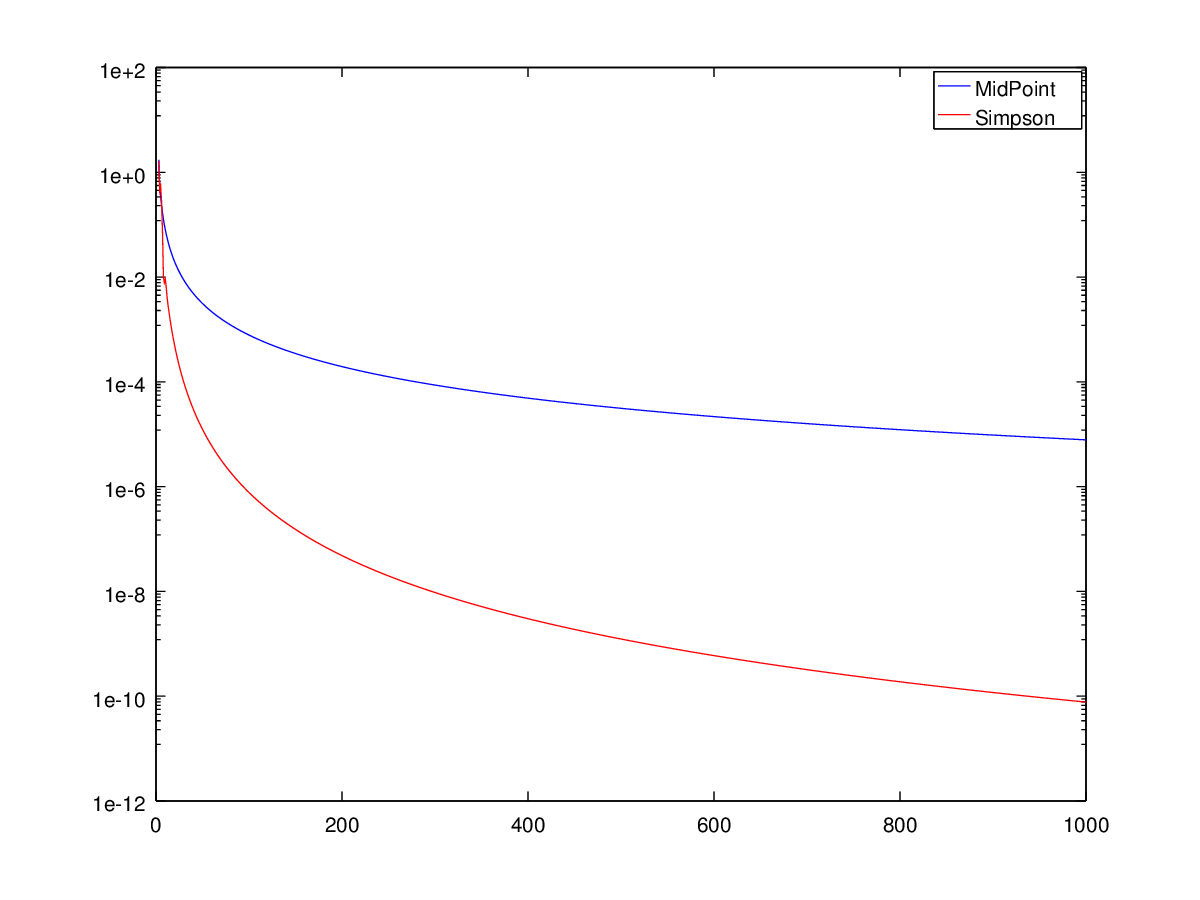
\includegraphics[scale=0.7]{quadrature}
\end{center}
\end{document}
